\documentclass{beamer}

% Beamer style
%\usetheme[secheader]{Madrid}
\usetheme{CambridgeUS}
\usecolortheme[rgb={0.65,0.15,0.25}]{structure}
%\usefonttheme[onlymath]{serif}
\beamertemplatenavigationsymbolsempty
%\AtBeginSubsection

% Packages
%\usepackage[french]{babel}
\usepackage[latin1]{inputenc}
\usepackage{color}
\usepackage{dsfont, stmaryrd}
\usepackage{amsmath, amsfonts, amssymb}
\usepackage{stmaryrd}
\usepackage{epsfig}
\usepackage{/Latex/astats}
%\usepackage[all]{xy}
\usepackage{graphicx}

% Commands
\definecolor{darkred}{rgb}{0.65,0.15,0.25}
\newcommand{\emphase}[1]{\textcolor{darkred}{#1}}
\newcommand{\paragraph}[1]{\emphase{#1}}
\newcommand{\refer}[1]{\textcolor{blue}{\sl \cite{#1}}}
\newcommand{\newblock}{}

% Symbols
\newcommand{\Abf}{{\bf A}}
\newcommand{\Beta}{\text{B}}
\newcommand{\Bcal}{\mathcal{B}}
\newcommand{\BIC}{\text{BIC}}
\newcommand{\dd}{\text{d}}
\newcommand{\dbf}{{\bf d}}
\newcommand{\Dcal}{\mathcal{D}}
\newcommand{\Esp}{\mathbb{E}}
\newcommand{\Ebf}{{\bf E}}
\newcommand{\Ecal}{\mathcal{E}}
\newcommand{\Gcal}{\mathcal{G}}
\newcommand{\Ibb}{\mathbb{I}}
\newcommand{\ICL}{\text{ICL}}
\newcommand{\Cov}{\mathbb{C}\text{ov}}
\newcommand{\Var}{\mathbb{V}}
\newcommand{\Vsf}{\mathsf{V}}
\newcommand{\pen}{\text{pen}}
\newcommand{\Hbf}{{\bf H}}
\newcommand{\Hcal}{\mathcal{H}}
\newcommand{\Jcal}{\mathcal{J}}
\newcommand{\Kbf}{{\bf K}}
\newcommand{\Lcal}{\mathcal{L}}
\newcommand{\Mcal}{\mathcal{M}}
\newcommand{\mbf}{{\bf m}}
\newcommand{\mum}{\mu(\mbf)}
\newcommand{\Ncal}{\mathcal{N}}
\newcommand{\Nbf}{{\bf N}}
\newcommand{\Nm}{N(\mbf)}
\newcommand{\Ocal}{\mathcal{O}}
\newcommand{\Obf}{{\bf 0}}
\newcommand{\Omegas}{\underset{s}{\Omega}}
\newcommand{\Pbf}{{\bf P}}
\newcommand{\Pcal}{\mathcal{P}}
\newcommand{\Qcal}{\mathcal{Q}}
\newcommand{\Rbb}{\mathbb{R}}
\newcommand{\Rcal}{\mathcal{R}}
\newcommand{\Ucal}{\mathcal{U}}
\newcommand{\Vcal}{\mathcal{V}}
\newcommand{\Tbf}{{\bf T}}
\newcommand{\Ubf}{{\bf U}}
\newcommand{\xbf}{{\bf x}}
\newcommand{\Xbf}{{\bf X}}
\newcommand{\Ybf}{{\bf Y}}
\newcommand{\Zbf}{{\bf Z}}
\newcommand{\pibf}{\mbox{\mathversion{bold}{$\pi$}}}
\newcommand{\Sigmabf}{\mbox{\mathversion{bold}{$\Sigma$}}}
\newcommand{\gammabf}{\mbox{\mathversion{bold}{$\gamma$}}}
\newcommand{\mubf}{\mbox{\mathversion{bold}{$\mu$}}}
\newcommand{\nubf}{\mbox{\mathversion{bold}{$\nu$}}}
\newcommand{\thetabf}{\mbox{\mathversion{bold}{$\theta$}}}
\newcommand{\BP}{\text{BP}}
\newcommand{\EM}{\text{EM}}
\newcommand{\VEM}{\text{VEM}}
\newcommand{\VBEM}{\text{VB}}
\newcommand{\cst}{\text{cst}}
\newcommand{\obs}{\text{obs}}


%====================================================================
\title[Biological Network]{Statistical Inference for Biological
  Interaction Networks}

\author{S. Robin}

\institute[AgroParisTech / INRA]{AgroParisTech / INRA \\
  \bigskip
  \begin{tabular}{ccccc}
    
\epsfig{file=../Figures/LogoINRA-Couleur.ps, width=2.5cm} &
    \hspace{.5cm} &
    
\epsfig{file=../Figures/logagroptechsolo.eps, width=3.75cm} &
    \hspace{.5cm} &
    \epsfig{file=../Figures/Logo-SSB.eps, width=2.5cm} \\
  \end{tabular} \\
  \bigskip
  }

\date{Lille, May 2010}
%====================================================================

%====================================================================
%====================================================================
\begin{document}
%====================================================================
%====================================================================

%====================================================================
\frame{\titlepage}
%====================================================================

%====================================================================
\frame{ \frametitle{Outline}
%==================================================================== 
  %\settocdepth[1]
  \tableofcontents
  }

%====================================================================
%====================================================================
\section{Interaction Networks}
\subsection*{Biological Networks}
\frame{ \frametitle{Some interaction networks}
%==================================================================== 
  \hspace{-1cm}
  \begin{tabular}{cc}
    \begin{tabular}{p{6cm}}
      \begin{itemize}
      \item \paragraph{Social networks:} Who loves who?  Who's friend
        with who?
      \item \paragraph{Industrial/commercial networks:} Number of
        passenger between airports.
      \item \paragraph{Internet:} Hyperlinks between websites.
      \item \paragraph{Biological networks:}
        Gene regultaion. Protein-protein interaction. \\
        Species sharing parasites.
      \end{itemize}
    \end{tabular}
    &
    \begin{tabular}{p{5cm}}
      \epsfig{file = ../Figures/Barabasi6.ps, clip=, bbllx=39, bblly=466,
        bburx=351, bbury=754, width=.5\textwidth, height=.7\textheight}
    \end{tabular}
  \end{tabular}
  }

%==================================================================== 
\frame{ \frametitle{Some statistical questions}
  \paragraph{Network inference:} \\
  Inferring the edges based on data observed at each nodes \\
  \emphase{$\rightarrow$} Gaussian graphical models

  \bigskip
  \paragraph{Modelling network evolution:} How the network has been
  build? \\
  \emphase{$\rightarrow$} Duplication/Mutation model for biological networks

  \bigskip
  \paragraph{Regression / Learning:} \\
  Which covariates contribute to explain the existence of a link?  \\
  Can we predict the existence of a link?  

  \bigskip
  \paragraph{Understanding/modelling network topology:} \\
  \emphase{$\rightarrow$} Global topology: Random graph models \\
  \emphase{$\rightarrow$} Local topology: Distribution of network motifs
  }

%==================================================================== 
\subsection*{Some models}
\frame{ \frametitle{Notations}
%==================================================================== 
  \paragraph{Random graph:} 
  \begin{itemize}
  \item Fix set of nodes: $ i \in  \{1, ... n\}$ 
  \item Linked by random edges: $\Xbf = \{X_{ij}\}_{i, j}$
  \end{itemize}
  It is characterised by the distribution
  $$
  P(\Xbf) = P(\{X_{ij}\}).
  $$

  \bigskip
  \paragraph{Topological characteristics:}
  \begin{itemize}
  \item node degrees (scale-free distribution?), 
  \item network diameter (small-world effect?),
  \item number of triangles and/or the clustering coefficient,
  \item number of connected components and the size of the largest
    one.
  \end{itemize}
  }

%==================================================================== 
\frame{ \frametitle{Some models}
  \paragraph{Erd�s \& R�nyi:} $\{X_{ij}\}_{1 \leq i < j \leq n}$ i.i.d.
  $$
  X_{ij} \sim \Bcal(\gamma)
  $$
  Preserves the density of the network, \\
  but not other characteristics of most real network.
  
  \bigskip  \bigskip
  \paragraph{Fix degree distribution (FDD):} $k_i =$ degree of node $i$, 
  $$
  \Xbf \sim \Ucal\{\xbf: \sum_j x_{ij} = k_i\}
  $$
  Preserves the degree of each node, \\
  but sampling such graphs is not that easy (edge swapping algorithm).

  \bigskip  \bigskip
  \paragraph{Statistical inference:} Easy in both cases. 
  }

%==================================================================== 
\frame{ \frametitle{Some models (cont'd)}
  \paragraph{Latent space models (\refer{BJR07}):} $\Zbf = \{Z_i\}$
  latent positions 
  \begin{eqnarray*}
    \{Z_i\} \text{ i.i.d. } & \sim & \pi \\
    \{X_{ij}\} \text{ independent } | \{Z_i\}: X_{ij}  & \sim &
    \Bcal[\gamma(Z_i, Z_j)]
  \end{eqnarray*}
  \paragraph{Continuous (\refer{HRH02}):} 
  $$
  Z_i \in \Rbb^k, \qquad \text{logit}[\gamma(z, z')] = a - |z-z'|
  $$
  \paragraph{Discrete (\refer{NoS01}):} 
  $$
  Z_i \in \{1, \dots, K\}, \qquad \gamma(k, \ell) = \gamma_{k\ell}.
  $$

  \bigskip\bigskip
  \paragraph{And also...}
  \begin{itemize}
  \item Preferential attachment
  \item Exponential random graphs models (ERGM)
  \item etc.  (\refer{PaR07})
  \end{itemize}
  }

%====================================================================
%====================================================================
\section{Mixture Model for Random Graphs}
\subsection*{Mixture Model}
\frame{ \frametitle{Mixture Model} \pause
%==================================================================== 
  \paragraph{Discrete-valued latent labels:}
  each node $i$ belong to class $q$ with probability $\pi_q$:
  $$
  \{Z_i\}_i \mbox{ i.i.d.}, \qquad Z_i \sim \Mcal(1; \pibf)
  $$
  where $\pibf = (\pi_1, \dots \pi_K)$;

  \bigskip
  \paragraph{Observed edges:} $\{X_{ij}\}_{i,
    j}$ are conditionally independent given the $Z_i$'s:
  $$
  (X_{ij} \;|\; Z_i = k, Z_j = \ell) \sim f_{k\ell}(\cdot).
  $$
  where $f_{k\ell}(\cdot)$ is some parametric distribution
  $f_{k\ell}(x) = f(x; \gamma_{k\ell})$, e.g.
  $$
  (X_{ij}|Z_{ik}Z_{j\ell}=1) \sim \Bcal(\gamma_{k\ell})
  $$
  We denote   $\gammabf = \{\gamma_{k\ell}\}_{k, \ell}.$
  
  \bigskip
  \paragraph{Inference:} We need to estimate
  $$
  \thetabf = (\pibf, \gammabf)
  \qquad \text{and} \qquad
  P(Z_i | \Xbf)
  $$
  }

%==================================================================== 
\frame{ \frametitle{Illustration: A social network}
%   \vspace{-1cm}\hspace{-1cm}
%   \begin{tabular}{cc}
%     \begin{tabular}{p{.5\textwidth}}
%       \paragraph{Data.} Social binary network of friendship within a
%       sport club. \\
%       \\
%       \paragraph{Results.} 
%       The split is recovered and the role of the leaders is underlined. 
%     \end{tabular}
%     &
%     \begin{tabular}{p{.5\textwidth}}
%       {\small
%         \begin{tabular}{c|rrrr}
%           & \multicolumn{4}{c}{$\widehat{\gamma}_{k\ell}$ (\%)} \\
%           $k / \ell$ &  {1} & 2 & 3 &  4 \\
%           \hline
%           {1} &  {100} &   {53} &  {16} & {16} \\  
%           {2} & - &  {12} & {0} & {7}  \\  
%           3 & - & - & 8 & 73 \\
%           4 & - & - & - & 100\\
%           \hline
%           $n\pi_{\ell}$        & 3 &  13       & 16    & 2     \\
%         \end{tabular}
%         }
%     \end{tabular}
%     \\
%     \\
%     \begin{tabular}{p{.5\textwidth}}
%       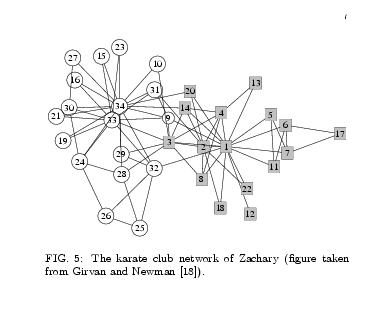
\epsfig{file=../Figures/graphe_karate.ps, clip=, bbllx=93,
%         bblly=140, bburx=550, bbury=440, width=.4\textwidth}
%     \end{tabular}
%     &
%     \begin{tabular}{p{.5\textwidth}}
%       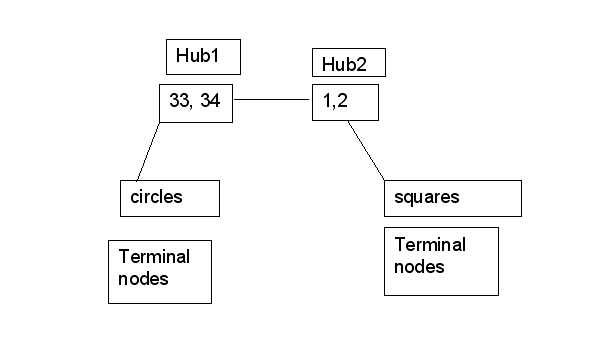
\epsfig{file=../Figures/karate-simple.ps, width=.4\textwidth, clip=,
%         bbllx=117, bblly=70, bburx=505, bbury=324}
%     \end{tabular}
%   \end{tabular}
  \vspace{-1cm}\hspace{-1cm}
  \begin{tabular}{c}
    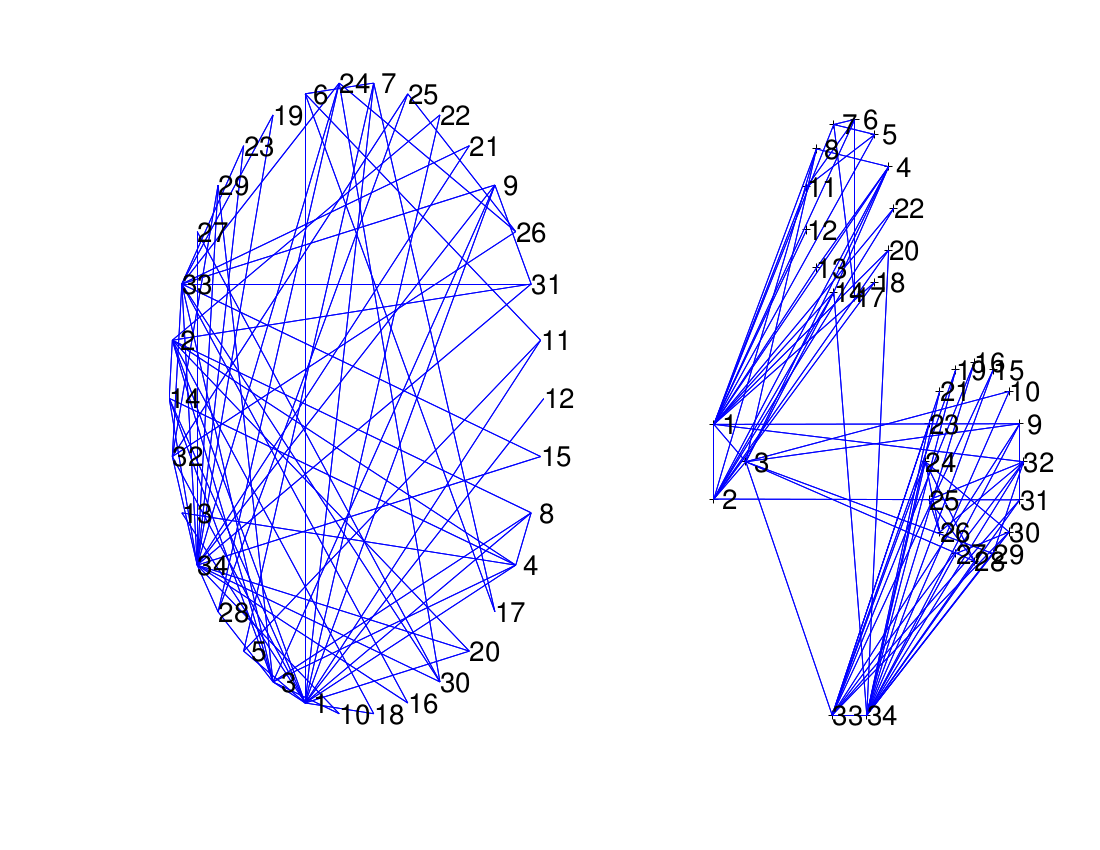
\epsfig{file = ../Figures/Karate-Graph.eps, clip=, width=3.5cm,
      height=10cm, angle=270}
    \\
    \\
    \begin{tabular}{cc}
      \begin{tabular}{p{.45\textwidth}}
        \paragraph{Data.} Social binary network of friendship within a
        sport club. \\
        \\
        \paragraph{Results.} 
        The split is recovered and the role of the leaders is underlined. 
      \end{tabular}
      &
      \begin{tabular}{p{.5\textwidth}}
        {\small
          \begin{tabular}{c|rrrr}
            & \multicolumn{4}{c}{$\widehat{\gamma}_{k\ell}$ (\%)} \\
            $k / \ell$ &  {1} & 2 & 3 &  4 \\
            \hline
            {1} &  {100} &   {53} &  {16} & {16} \\  
            {2} & - &  {12} & {0} & {7}  \\  
            3 & - & - & 8 & 73 \\
            4 & - & - & - & 100\\
            \hline
            $n\pi_{\ell}$        & 3 &  13       & 16    & 2     \\
          \end{tabular}
          }
      \end{tabular}
    \end{tabular}
  \end{tabular}
  }

%==================================================================== 
\subsection*{Variational Inference}
\frame{ \frametitle{Maximum likelihood inference}
%==================================================================== 
  \paragraph{Maximum likelihood estimate:} We are looking for
  $$
  \widehat{\thetabf} = \arg\max_{\thetabf} \log P(\Xbf; \thetabf)
  $$

  \paragraph{Incomplete data model:}
  \begin{itemize}
  \item The calculation of
    $$
    P(\Xbf; \thetabf) = \sum_{\Zbf} P(\Xbf, \Zbf; \thetabf)
    $$
    is not always possible since this sum typically involves $K^n$ terms.
  \item This of 
    $$
    P(\Xbf, \Zbf; \thetabf)
    $$
    is much easier ... except that {$\Zbf$ is unknown}.
  \end{itemize}
  }

%====================================================================
\subsection*{Variational approach}
\frame{ \frametitle{Variational approach}
%==================================================================== 
  \paragraph{Lower bound of the likelihood:}
  For any distribution $Q(\Zbf)$, we have [\refer{JGJ99,Jaa00}]
  \begin{eqnarray*}
    \log P(\Xbf) & \geq & \log P(\Xbf) - KL[Q(\Zbf); P(\Zbf|\Xbf)] \\
%     & = & \log P(\Xbf) - \int Q(\Zbf) \log Q(\Zbf) \dd\Zbf + \int
%     Q(\Zbf) \log \emphase{P(\Zbf |\Xbf)} \dd\Zbf \\   
%     & = & - \int Q(\Zbf) \log Q(\Zbf) \dd\Zbf + \int Q(\Zbf) \log
%     \emphase{P(\Xbf, \Zbf)} \dd\Zbf \\
    & = & \Hcal(Q) + \Esp_Q[\log P(\Xbf, \Zbf)].
  \end{eqnarray*}
  where
  \begin{eqnarray*}
    \Hcal(Q) & = & \int Q(\Zbf) \log Q(\Zbf) \dd\Zbf \\
    \Esp_Q[\log P(\Xbf, \Zbf)] & = & \int Q(\Zbf) \log \emphase{P(\Xbf, \Zbf)} \dd\Zbf
  \end{eqnarray*}
  }

%==================================================================== 
\frame{ \frametitle{Consequences}
  \paragraph{If $P(\Zbf|\Xbf)$ can be calculated}: taking $Q(\Zbf) =
  P(\Zbf|\Xbf)$ achieves the maximisation of $\log P(\Xbf)$ through
  this of
  $$
  \Esp_Q[\log P(\Xbf, \Zbf; \thetabf)].
  $$
  \emphase{$\rightarrow$} E-M algorithm for independent mixtures, hidden
  Markov models, etc. %[\refer{DLR77,MaP00,CMR05}].
  
  \bigskip\bigskip
  \paragraph{If $P(\Zbf|\Xbf)$ can not be calculated}: the best lower
  bound of $\log P(\Xbf)$ is obtained for
  $$
  Q^* = \arg\min_{Q \in \Qcal} KL[Q(\Zbf); P(\Zbf|\Xbf)]
  $$
  \emphase{$\rightarrow$} Mean-field approximation for random graphs.
  }

%====================================================================
\subsection*{Variational E-M}
\frame{ \frametitle{Variational E-M}
%==================================================================== 
  \paragraph{'Expectation' step (E-step):} calculate
  $$
  P(\Zbf|\Xbf; \thetabf)
  $$
  or its approximation
  $$
  Q^* = \arg\min_{Q \in \Qcal} KL[Q(\Zbf); P(\Zbf|\Xbf; \thetabf)].
  $$

  \bigskip
  \paragraph{Maximisation step (M-step):} estimate $\thetabf$ with
  $$
  \widehat{\thetabf} = \arg\max_{\thetabf} \Esp_Q[\log P(\Xbf, \Zbf; \thetabf)]
  $$
  which maximise $\log P(\Xbf)$ if $Q(\Zbf) = P(\Zbf|\Xbf)$, and its
  lower bound otherwise.
  }

%==================================================================== 
\frame{ \frametitle{Dependency structure}
  \begin{tabular}{c|c|c}
    \begin{tabular}{p{.28\textwidth}}
      \emphase{Graphical rep.:} \\ 
      $P(\Zbf) P(\Xbf|\Zbf)$
    \end{tabular}
    &
    \begin{tabular}{p{.28\textwidth}}
      \emphase{Moral graph}  \\
      (\refer{Lau96})
    \end{tabular}
    &
    \begin{tabular}{p{.28\textwidth}}
      \emphase{Cond. dependency:} \\ 
      $P(\Zbf|\Xbf)$
    \end{tabular}
    \\
    \hline
    & & \\
    \begin{tabular}{c}
      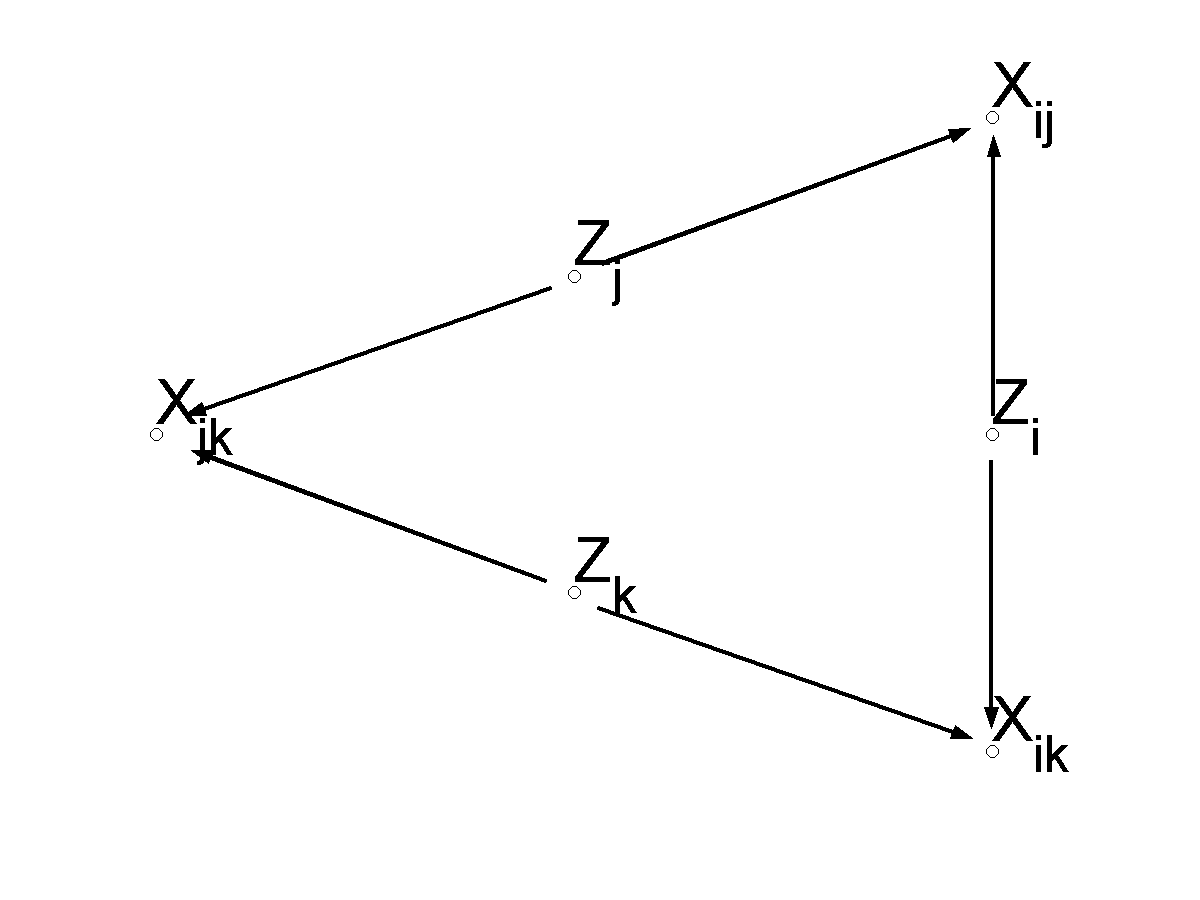
\epsfig{file=../Figures/FigNetworks-DepGraph,
      width=.25\textwidth, clip=} 
    \end{tabular}
    & 
    \begin{tabular}{c}
      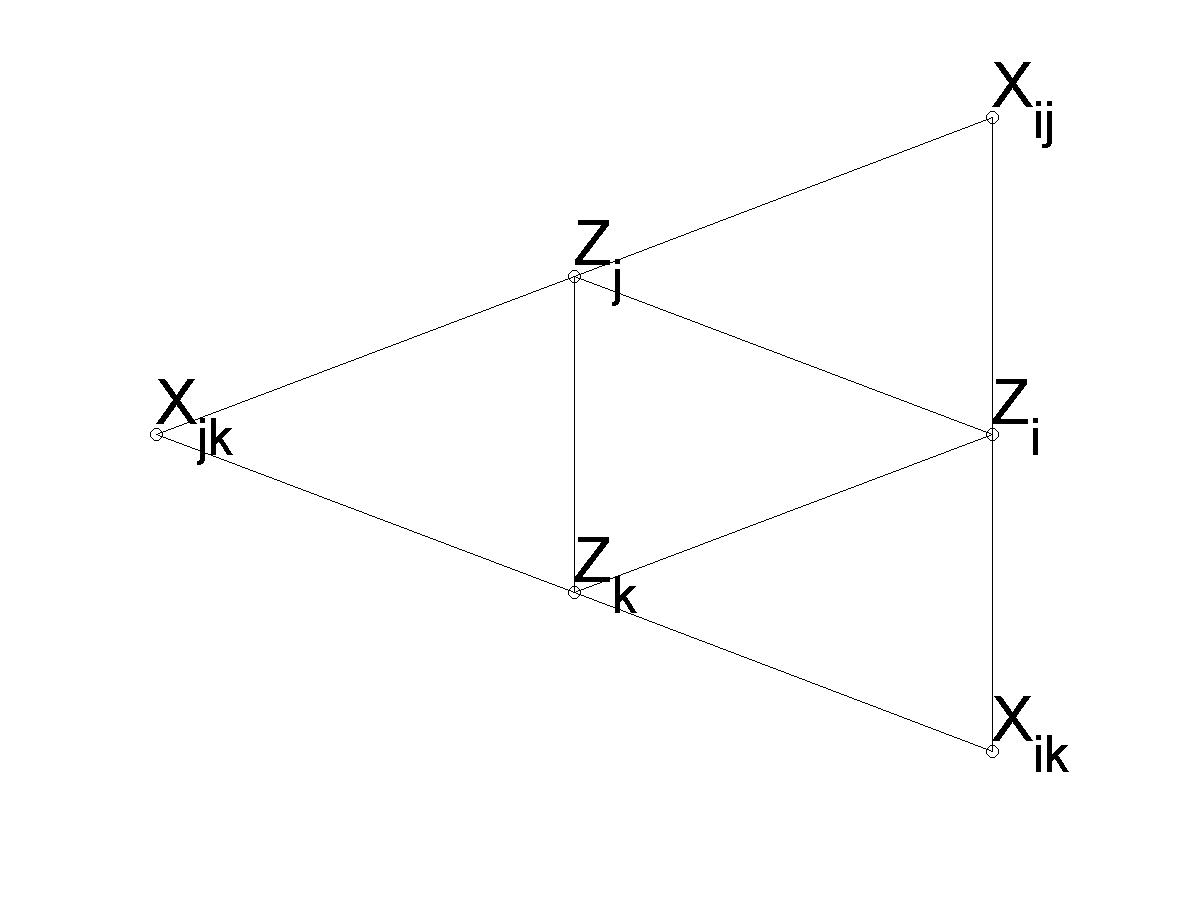
\epsfig{file=../Figures/FigNetworks-DepGraph-Moral,
      width=.25\textwidth, clip=}
    \end{tabular}
    & 
    \begin{tabular}{c}
      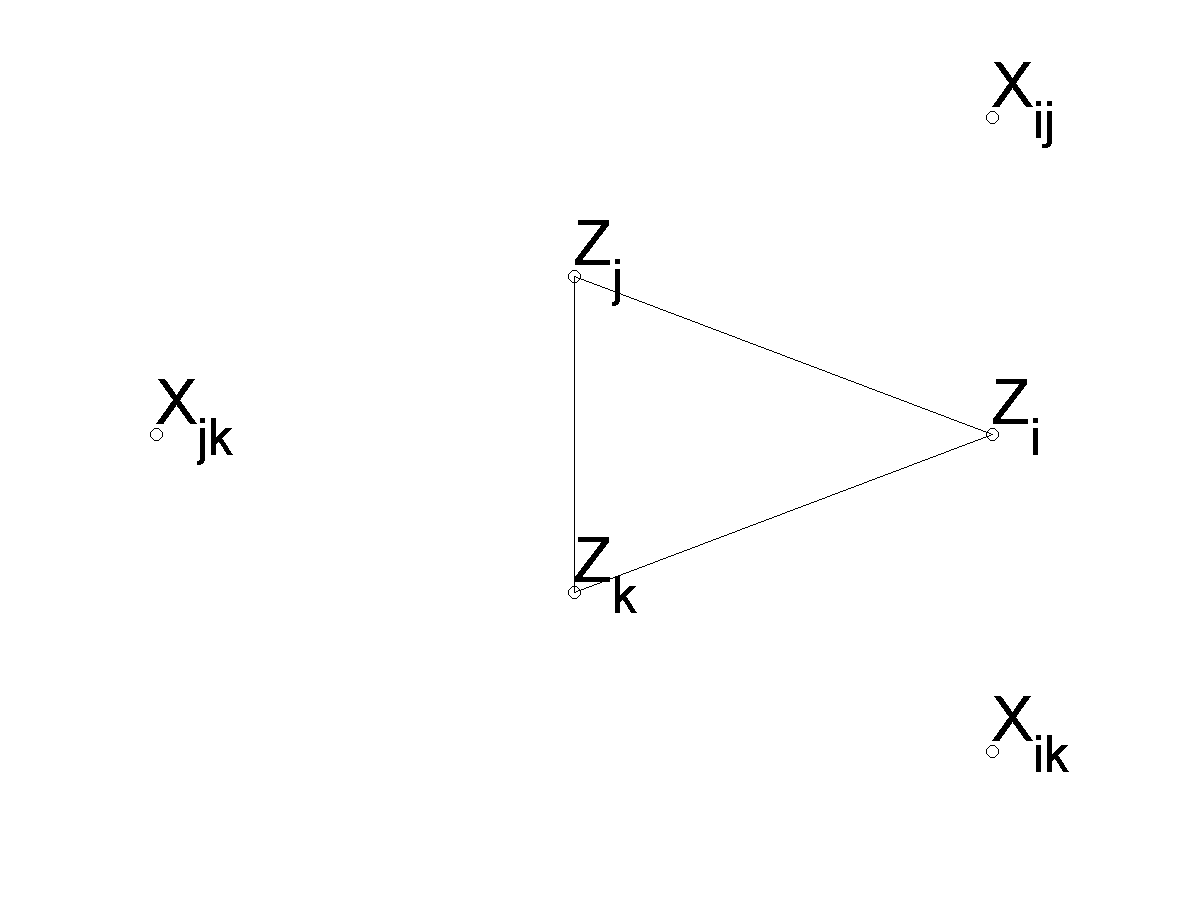
\epsfig{file=../Figures/FigNetworks-DepGraph-Conditional,
      width=.25\textwidth, clip=}
    \end{tabular} 
  \end{tabular}

  \bigskip\bigskip
  The conditional dependency of $\Zbf$ is a \emphase{clique} \\
  \emphase{$\rightarrow$} no factorisation can be hoped to calculate
  $P(\Xbf|\Zbf)$ \\
  \emphase{$\rightarrow$} $P(\Xbf|\Zbf)$ can {only be approximated}.
  }
%====================================================================
\subsection*{Inference}
\frame{ \frametitle{Likelihood}
%==================================================================== 
  \paragraph{Complete likelihood:}
  $$
  \log P(\Xbf, \Zbf) = \sum_{i, k} Z_{ik} \log \pi_k + \sum_{i, j}
  \sum_{k, \ell} Z_{ik} Z_{j\ell} \log f(X_{ij}; \gamma_{k\ell}).
  $$
   
  %\bigskip
   \paragraph{Completed likelihood:} 
   $$
   \Esp_Q[\log P(\Xbf, \Zbf)] = \sum_{i, k}
   \underset{\emphase{\normalsize
       \tau_{ik}}}{\underbrace{\Esp_Q[Z_{ik}]}} \log \pi_k + \sum_{i,
     j} \sum_{k, \ell} \Esp_Q[Z_{ik} Z_{j\ell}]  \log f(X_{ij};
   \gamma_{k\ell}). 
   $$
   
   ~\\
   \paragraph{M-step:} weighted version of the MLE.  
   }

%====================================================================
\frame{ \frametitle{Approximation of $P(\Zbf|\Xbf)$}
  \paragraph{Problem:}  
  We are looking for
  $$
  Q^* = \arg\min_{Q \in \Qcal} KL[Q(\Zbf); P(\Zbf|\Xbf)].
  $$

  \begin{itemize}
%   \item The optimum over all possible distributions is
%     \emphase{$Q^*(\Zbf) = P(\Zbf|\Xbf)$} ... which can no be
%     calculated.
  \item We restrict ourselves to the set of \emphase{factorisable
      distributions}:
    $$
    \Qcal = \left\{Q: Q(\Zbf) = \prod_i Q_i(Z_i) = \prod_i \prod_k
      \tau_{ik}^{Z_{ik}}\right\}. 
    $$
    $Q^*$ is characterised by the set of optimal parameters
    $\tau_{ik}^*$'s:
    $$
    \emphase{\tau_{ik}^* = \Esp_Q[Z_{ik}] \approx \Pr\{Z_i=k|\Xbf\}}.
    $$
  \item The optimal $\tau_{ik}^*$'s can be found using {standard
    (constrained) optimisation} techniques.
  \end{itemize}
  }
    
%====================================================================
\frame{ \frametitle{Best factorisable approximation}
  The optimal $\tau_{ik}$'s must satisfy
%   $$
%   \left.\frac{\partial}{\partial
%       \tau_{ik}}\right|_{\{\tau_{ik}^*\}} \left\{KL[Q(\Zbf);
%     P(\Zbf|\Xbf)] + \sum_i \lambda_i \left(\sum_{k} \tau_{ik} -
%       1\right)\right\} = 0
%   $$
%   which leads to 
  the {fix-point relation}:
  $$
  \tau_{ik}^* \propto \pi_k \prod_{j \neq i} \prod_\ell
%   \left[\gamma_{k\ell}^{X_{ij}} (1 -
%     \gamma_{k\ell})^{1-X_{ij}}\right]^{\emphase{\tau^*_{j\ell}}}
  f_{k\ell}(X_{ij})^{\emphase{\tau^*_{j\ell}}}
  $$
  also known as \emphase{mean-field} approximation in physics.

  \bigskip
  \paragraph{Intuitive interpretation:}
  $$
  \Pr\{Z_i=k | \Xbf, \Zbf_{\emphase{\setminus i}}\} \propto \pi_k
%   \prod_{j \neq i} \prod_\ell \left[\gamma_{k\ell}^{X_{ij}} (1 -
%     \gamma_{k\ell})^{1-X_{ij}}\right]^{\emphase{Z_{j\ell}}}.
  \prod_{j \neq i} \prod_\ell
  f_{k\ell}(X_{ij})^{\emphase{Z_{j\ell}}}. 
  $$

  \bigskip
  \paragraph{Improvement:} The approximation of $\Esp_Q[Z_{ik}
  Z_{j\ell}]$ can be improved via a \emphase{message passing
    algorithm}.  
  }

%==================================================================== 
\frame{ \frametitle{Some more statistical issues}
  \paragraph{Choice of $K$}
  \begin{itemize}
  \item Usual BIC requires the calculation of $P(\Xbf)$;
  \item ICL only requires this of $\Esp_Q[P(\Xbf, \Zbf)]$.
  \end{itemize}

  \bigskip
  \paragraph{Extension to variational Bayes inference}
  \begin{itemize}
  \item In a Bayesian context, $\thetabf$ can be viewed as an
    unobserved variable;
  \item Variational Bayes EM (VB-EM) aims at minimising
    $$
    KL[Q(\thetabf, \Zbf); P(\thetabf, \Zbf|\Xbf)]
    $$
  \end{itemize}

  \bigskip
  \paragraph{General properties of variational estimates.}
  \begin{itemize}
  \item Consistency of variational Bayes posterior mode in mixture
    models;
  \item Underestimation of the posterior variance.
  \end{itemize}

  \bigskip
  \paragraph{Special case of graphs}
  \begin{itemize}
  \item Specific asymptotic framework ($p = n$);
  \item Better quality of the mean-field approximation.
  \end{itemize}
  }

%====================================================================
\subsection*{Application to regulatory networks}
\frame{ \frametitle{Application to regulatory network}
%==================================================================== 
  \vspace{-.5cm}\hspace{-.5cm}
  \begin{tabular}{ll}
    \begin{tabular}{p{6cm}}
      Regulatory network = directed graph where
      \begin{itemize}
      \item \emphase{Nodes =} genes (or groups of genes, e.g. operons)
      \item \emphase{Edges =} regulations:
        $$
        \emphase{\{i \rightarrow j\}}
        \quad \Leftrightarrow \quad 
        \emphase{i \text{ regulates } j}
        $$
      \end{itemize}

      Typical questions are
      \begin{itemize}
      \item Do some nodes share similar connexion profiles?
      \item Is there a 'macroscopic' organisation of the network?
      \end{itemize}    
    \end{tabular}
    &
    \begin{tabular}{l}
      \hspace{-.75cm}
      \epsfig{file=/ENSEIGN/COURS/MELANGE/Exposes/Figures/im_EcoliVEM.ps,
      width=.45\textwidth, clip=} 
    \end{tabular}
  \end{tabular}
  }

%==================================================================== 
\frame{ \frametitle{Meta-graph representation}
  \hspace{-0.75cm}
  \begin{tabular}{cc}
    \begin{tabular}{p{0.45\textwidth}}
      \epsfig{file=/ENSEIGN/COURS/MELANGE/Exposes/Figures/im_EcoliVEM.ps,
      width=.45\textwidth, clip=} 
    \end{tabular}
    &
    \begin{tabular}{p{0.45\textwidth}}
      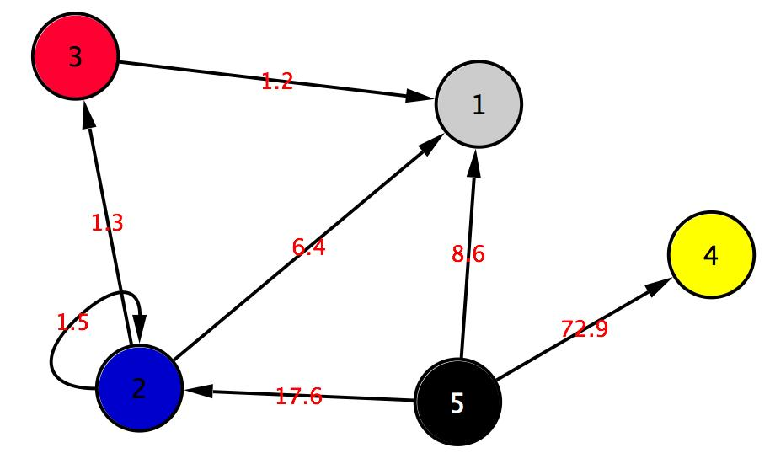
\epsfig{file=/ENSEIGN/COURS/MELANGE/Exposes/Figures/VEMmetagraphe.ps,
      width=.45\textwidth, clip=}  
      \\ \\
      \tiny{$\begin{array}{cccccc}
          \widehat{\gamma}_{k\ell}~(\%) & 1 & 2 & 3 & 4 & 5 \\
          \hline
          1 & . & . & . & . & . \\
          2 & 6.40 & 1.50 & 1.34 & . & . \\
          3 & 1.21 & . & . & . & . \\
          4 & . & . & . & . & . \\
          5 & 8.64 & 17.65 & . & 72.87 & 11.01 \\
          \hline
          \widehat{\alpha}~(\%) & 65.49 & 5.18 & 7.92 & 21.10 & 0.30
        \end{array}$}
      \\ \\
      (source \refer{PMD09})
    \end{tabular}
  \end{tabular}
  }

%====================================================================
%====================================================================
\section{Network Motifs}
\subsection*{Exceptionnal network Motifs}
\frame{ \frametitle{Network motifs (NeMo ANR project)} \pause
%==================================================================== 
  \hspace{-0.75cm}
  \begin{tabular}{ll}
    \begin{tabular}{p{0.8\textwidth}}
      \paragraph{Local patterns} constitute 
      {functional modules} or basic building
      blocks of complex networks (\refer{SMM02}). \\

      ~\\
      \paragraph{Transcription regulatory networks:} 
      motifs may perform specific regulatory functions
      (e.g. feed-forward loop, bi-fan: see right). \\

      ~\\
      \paragraph{Focus on exceptional motif}, i.e. appearing more
      {frequently than expected} that are thought to reflect
      {functional units} which combine to regulate the cellular
      behaviour. \\
      \refer{MSI02}, \refer{MaA03}, \refer{PIL05}
    \end{tabular}
    &
    \begin{tabular}{p{0.2\textwidth}}
      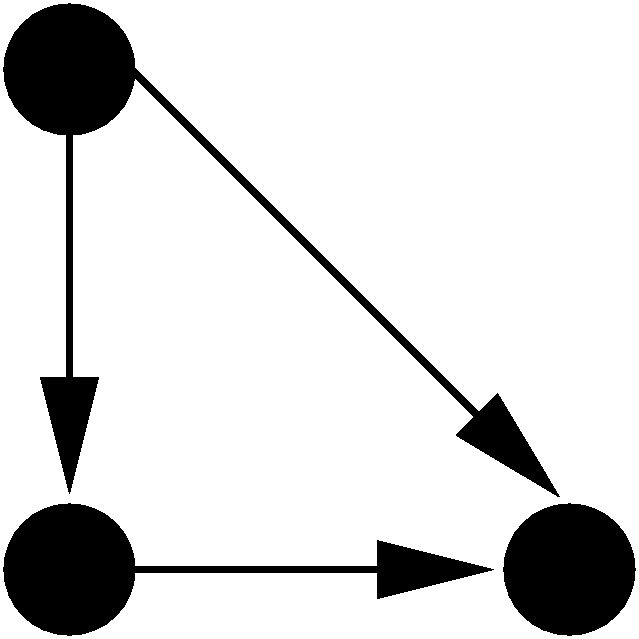
\epsfig{file=../Figures/feedforwardloop.eps, clip=,
        width=.1\textwidth} \\
      \\
      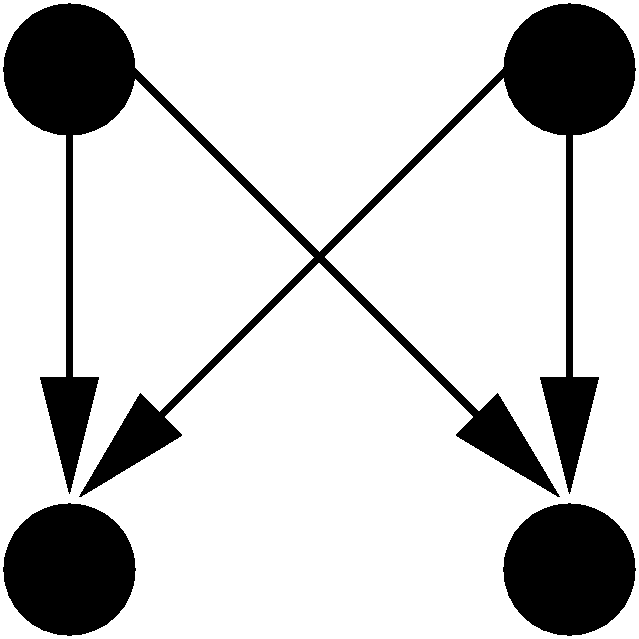
\epsfig{file=../Figures/bifan.eps, clip=, width=.1\textwidth}
    \end{tabular}
  \end{tabular}
  }


%==================================================================== 
\frame{ \frametitle{Assessing the exceptionality of a motif}
  \paragraph{For a given (relevant) random graph model}, we need to evaluate
  $$
  \Pr\{\Nm \geq N_{\obs}(\mbf)\}
  $$
  where $N_{\obs}(\mbf)$ is the number of occurrences of a given
  motif $\mbf$ in the network under study.
  
  \bigskip\bigskip
  \paragraph{Asymptotic distributions of $\Nm$:} Gaussian, Poisson, Compound
  Poisson
  \begin{itemize}
  \item Only {simple models} (Erd�s-R�nyi) or
    {simple motifs} (triangle) are considered, 
  \item with {restrictive} underlying hypotheses,
    depending on the structure of the motif itself.
  \end{itemize}
  
  \bigskip\bigskip
  \paragraph{Standard approach in bioinformatics:}
  Compute a $p$-value based on 'empirical' moments and/or 'empirical'
  distribution via simulations (\refer{SMM02}).  
  }

%==================================================================== 
\subsection*{Motif detection}
\frame{ \frametitle{Topological motif}
%==================================================================== 
  \paragraph{Definition.}  A topological motif $\mbf$ of is
  characterised by its adjacency matrix (also denoted by $\mbf$):
  $$
  m_{uv} = \Ibb\{u \sim v\}.
  $$

  \hspace{-0.7cm}
  \begin{tabular}{cc}
    \begin{tabular}{p{0.4\textwidth}}
      \paragraph{Permutations.} For a given motif $\mbf$, we need to
      consider the set $\Rcal(\mbf)$ of its permutations. \\
      \\
      \paragraph{Right:} the $\mathsf{V}$ motif may occure in 3 ways at a
      {fixed} position $\alpha = (i,j,k)$: \\
      \\
    \end{tabular}
    &
    \begin{tabular}{ccc}
      $\mbf$ &  $\mbf^{\prime}$ & $\mbf^{\prime \prime}$ \\
      & & \\
      $\tiny{\left[ \begin{array}{ccc} 
          0 & 1 & 1 \\ . & 0 & 0 \\ . & . & 0 
        \end{array} \right]}$  &
      $\tiny{\left[ \begin{array}{ccc} 
          0 & 1 & 0 \\ . & 0 & 1 \\ . & . & 0 
        \end{array} \right]}$ &
      $\tiny{\left[ \begin{array}{ccc} 
          0 & 0 & 1 \\ . & 0 & 1 \\ . & . & 0 
        \end{array} \right]} $ \\
      &&
      \\
      \epsfig{file=../Figures/version2.eps, width=0.1\textwidth} & 
      \epsfig{file=../Figures/version3.eps, width=0.1\textwidth} & 
      \epsfig{file=../Figures/version1.eps, width=0.1\textwidth} 
      \\
    \end{tabular}
  \end{tabular}

  }

%==================================================================== 
\frame{ \frametitle{Occurrence of a topological motif}
  \paragraph{Position.} A ($k$-)position $\alpha$ is a set of $k$
  different nodes taken is ascending order:
  $$
  \alpha = (i_1, ... i_k), \qquad i_1 < i_2 < ... < i_k.
  $$
  A graph of size $n$ contains \emphase{$\displaystyle{\binom{n}{k}}$
    positions}.
  
  \bigskip
  \paragraph{(Induced) occurrence.} $Y_{\alpha}(\mbf) = $ {binary variable}:
  $$
  Y_{\alpha}(\mbf) 
  = \Ibb\{\mbf \text{ occurs at } \alpha\}
  =\prod_{1 \leq u < v \leq k} (X_{i_ui_v})^{m_{uv}}.
  $$
  
  \bigskip
  \paragraph{Count.} The total number of occurrences is the sum over
  {all positions} and {all permutations}: 
  $$
  N(\mbf) = \sum_{\alpha} \sum_{\mbf' \in \Rcal(\mbf)} Y_{\alpha}(\mbf').
  $$
  }

%==================================================================== 
\frame{ \frametitle{Moments of the count}
  
  \paragraph{Two assumptions (\refer{PDK08}):} 
  \begin{enumerate}[(H1)]
  \item {Stationarity:}
    $$ 
    \Dcal(X_{i_1j_1}, \ldots, X_{i_{\ell}j_{\ell}}) = \Dcal
    (X_{i'_1j'_1}, \ldots, X_{i'_{\ell}j'_{\ell}}). 
    $$
  \item {Independence of disjoint occurrences:}
    $$
    Y_\alpha(\mbf) \perp Y_\beta(\mbf) \quad \text{ if } \quad \alpha
    \cap \beta =\emptyset.  
    $$
  \end{enumerate}

  \bigskip\bigskip
  \paragraph{Occurrence probability} 
  Thanks to (H1), $\Pr\{Y_\alpha=1\}$ does not depend on $\alpha$:
  $$
  \forall \alpha, \forall \mbf' \in \Rcal(\mbf), \qquad
  \Pr\{Y_{\alpha}(\mbf') = 1\} = \Pr\{Y_{\alpha}(\mbf) = 1\} = \mum.
  $$
  }

%==================================================================== 
\frame{ \frametitle{Moments of the count (cont'd)}
  \paragraph{Mean:} Straightforwardly
  $$
  \Esp N(\mbf) = \sum_{\alpha} \sum_{\mbf' \in \Rcal(\mbf)}
  \Esp Y_{\alpha}(\mbf') = \binom{n}{k} |\Rcal(\mbf)| \mum.
  $$

  \bigskip
  \paragraph{Variance:} Obtained via the calculation of $\Esp
  [N(\mbf)^2]$.
  \begin{eqnarray*}
    N^2(\mbf) & = & \sum_{\alpha, \beta \in I_k}
    \sum_{\mbf^\prime, \mbf''\in \mathcal{R}(\mbf)}
    Y_{\alpha}(\mbf')Y_{\beta}(\mbf'') \\
    & = & \sum_{s=0}^k \sum_{|\alpha \cap \beta| = s}
    \sum_{\mbf', \mbf'' \in \Rcal(\mbf)} Y_{\alpha \cup \beta}(\mbf'
    \Omegas \mbf'')
  \end{eqnarray*}
  where $\Omegas$ is the \emphase{overlapping operator} with $s$
  common nodes and $\mbf' \Omegas \mbf''$ is the \emphase{super-motif}
  made of two overlapping occurrences of $\mbf'$ and $\mbf''$.
  }

%==================================================================== 
\frame{ \frametitle{Moments of the count (cont'd)}
  \hspace{-0.5cm}
  \begin{tabular}{cc}
    \begin{tabular}{p{0.4\textwidth}}
      \paragraph{Super-motifs} are made of overlapping
      occurrences of equivalent versions of $\mbf$. \\
      \\ \\
      \paragraph{Enumeration.} The adjacency matrices of all
      super-motifs can be listed \emphase{automatically}. \\
%      \\
%       The algorithm consist in the systematic exploration of all $\mbf'
%       \Omegas \mbf''=$ 
%       $$
%       \left(\begin{array}{c|c|c}
%           \mbf'_{11} & \mbf'_{12} & \Obf \\
%           \hline
%           \mbf'_{21} & \max(\mbf'_{22}, \mbf''_{11}) &  \mbf''_{12} \\
%           \hline
%           \Obf  & \mbf''_{21} &  \mbf''_{22} \\
%         \end{array} \right).
%       $$
      \\ \\
      \paragraph{Right:} All $\mbf' \Omegas \mbf''$ with $s=3$
      for the 4 spike star motif: \\
      \centerline{\begin{tabular}{cc}
          \begin{tabular}{c} $\mbf = $ \end{tabular} & 
          \begin{tabular}{c} \hspace{-1cm}     
            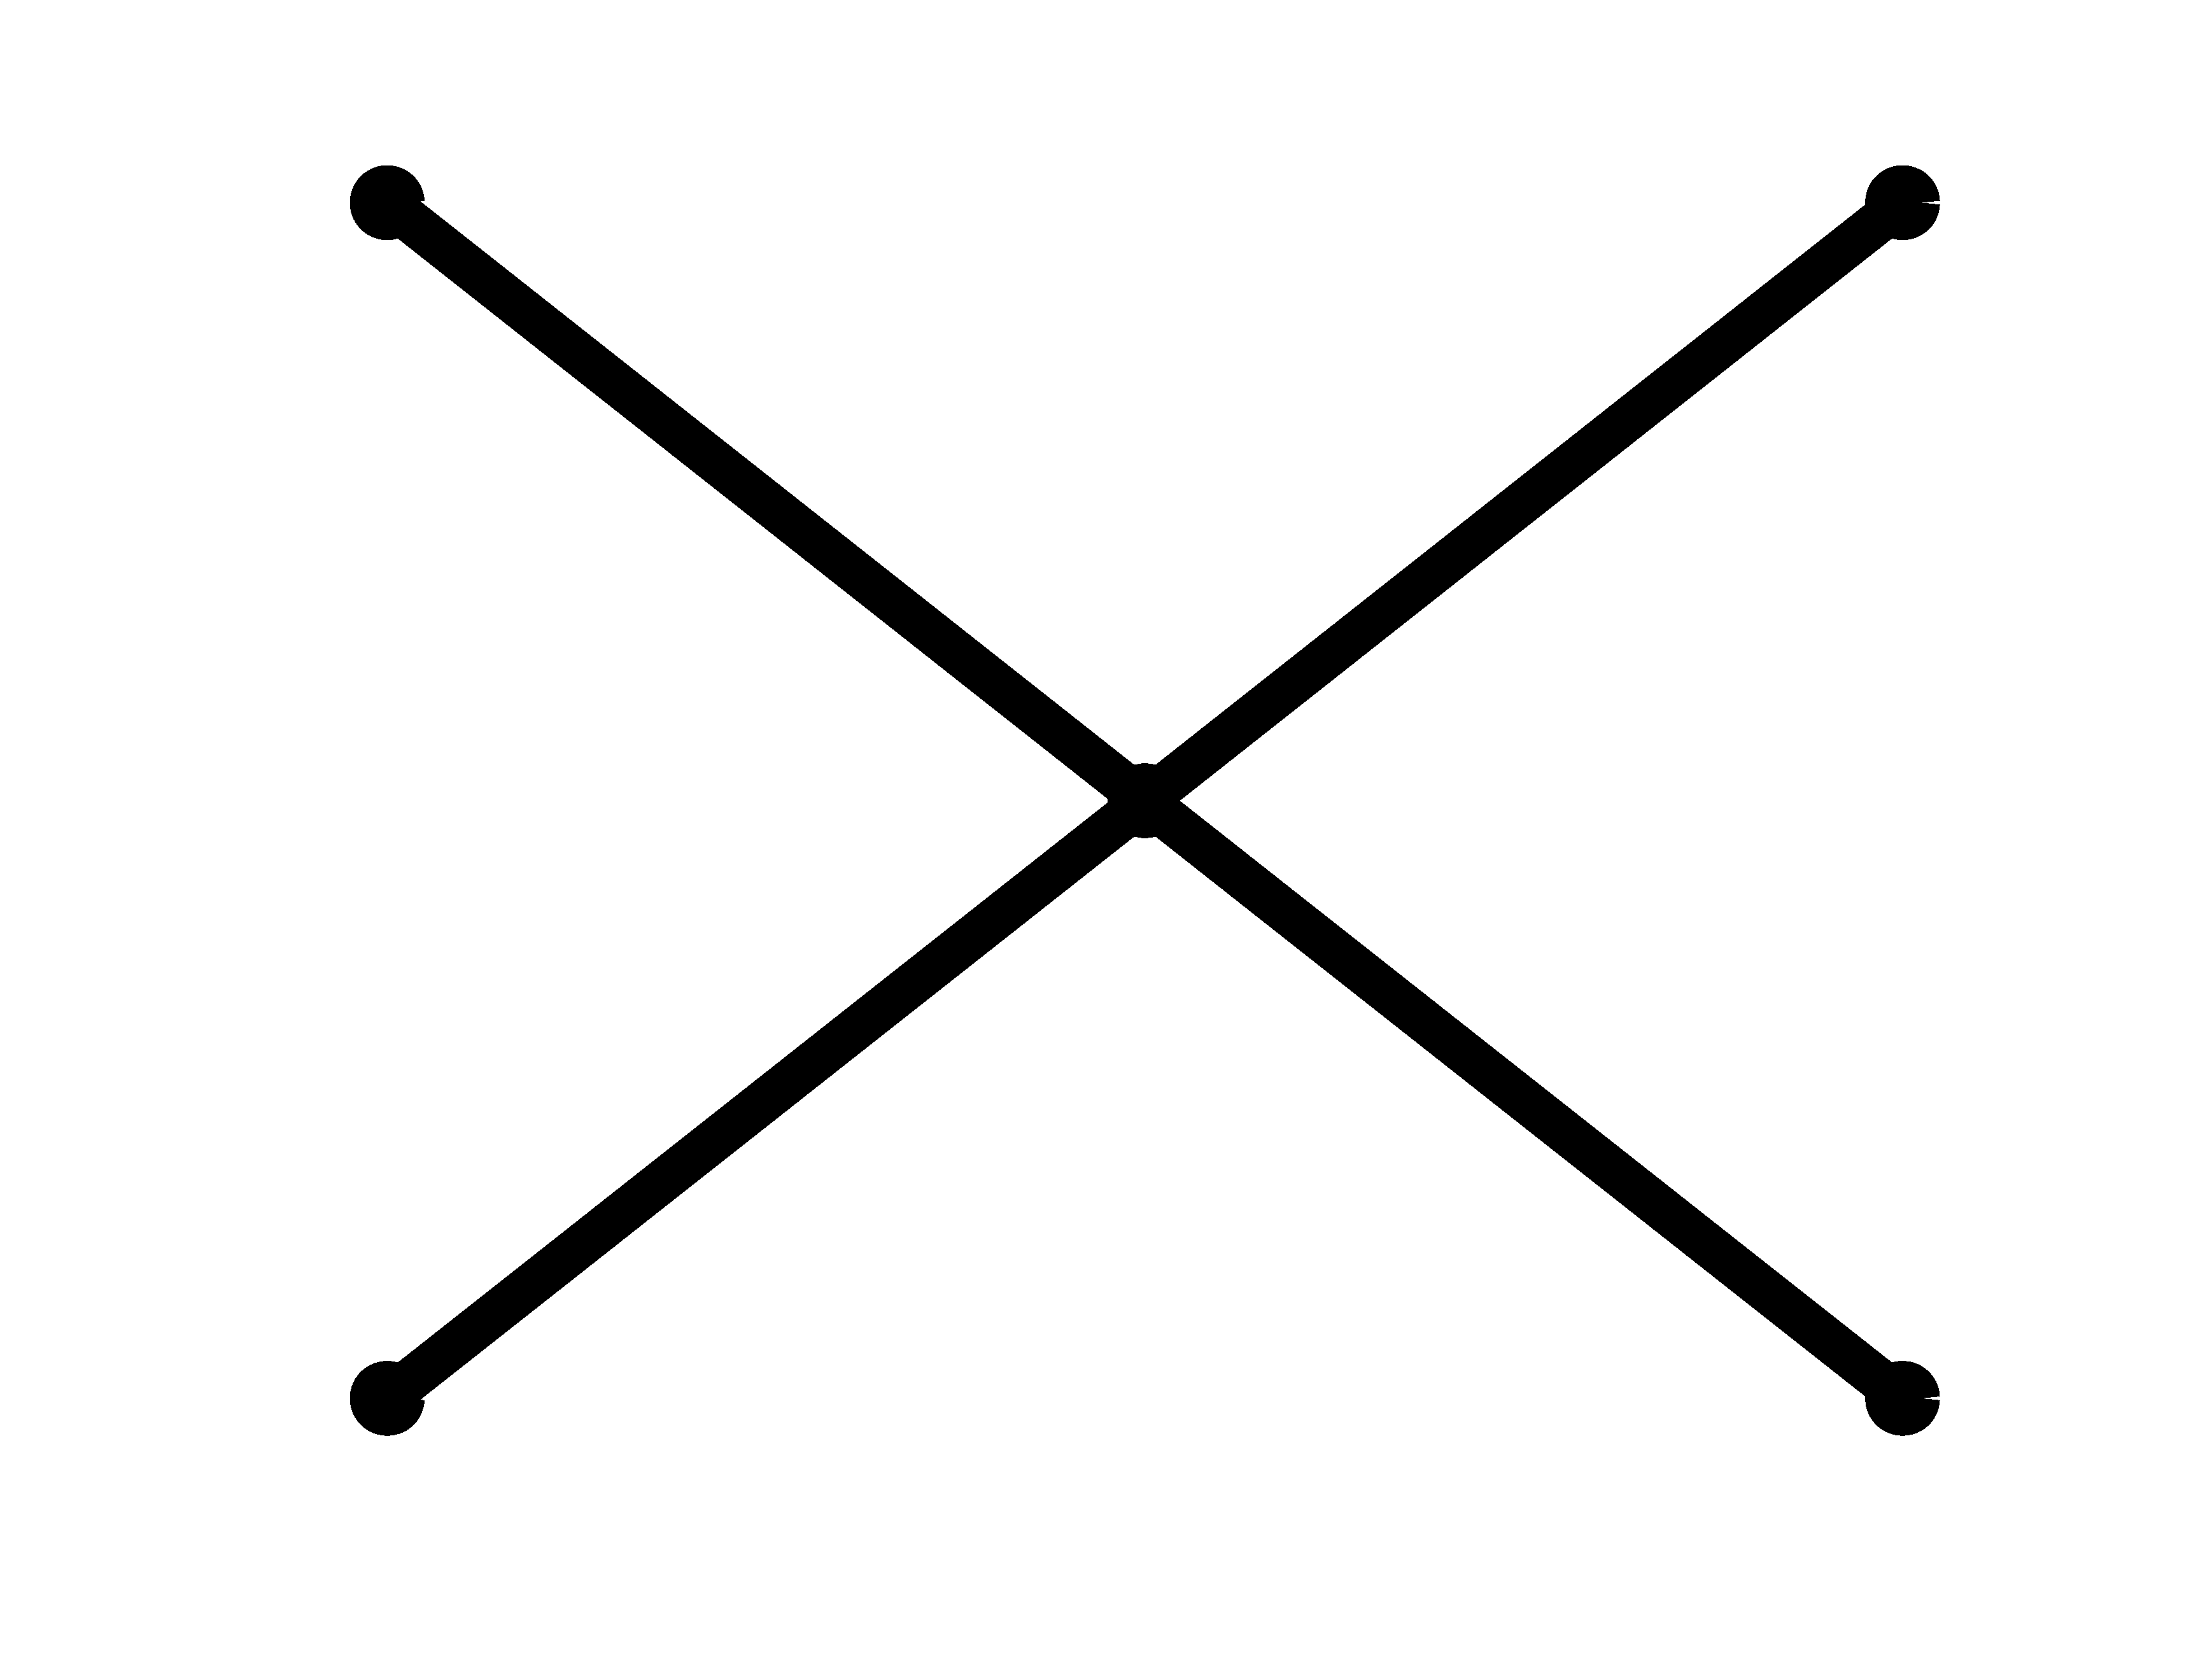
\epsfig{file = ../Figures/Motif-Star4.eps, clip=, 
              width=0.05\textwidth}
          \end{tabular}   
        \end{tabular}  } 
    \end{tabular}
    &
    \begin{tabular}{c}
      %\hspace{-1cm}
      \epsfig{file= ../../Motifs/FIGURES/MotifStar4-Recouv3.eps,
        clip=, width=0.5\textwidth, height=0.8\textheight}
    \end{tabular}
  \end{tabular}  
  }

%==================================================================== 
\frame{ \frametitle{Choosing the relevant graph model}
  \paragraph{Case of the FDD model:} The number of star motifs
  $\mbf_k$ (with $k$ arrows) is given by the degrees of the nodes
  $d_i$:
  $$
  N(\mbf_k) = \sum_i \binom{d_i}{k}
  \qquad \Rightarrow \qquad
  \left\{
    \begin{array}{rcl}
      \Esp_{FDD}[N(\mbf_k)] & = & N_{\obs}(\mbf_k), \\
      \\
      \Var_{FDD}[N(\mbf_k)] & = & 0.
    \end{array}
  \right.
  $$

  \bigskip
  \paragraph{Expected degree distribution (EDD) model.} $\dbf_{\obs} =
  \{d_i\}_i$ degrees in the observed graph;
    \begin{eqnarray*}
    \{K_i\}_i \text{ i.i.d. } & \sim & \Ucal\{\dbf_{\obs}\} \\
    \{X_{ij}\} \text{ independent } | \{Z_i\}: X_{ij}  & \sim &
    \Bcal(c K_i K_j)
  \end{eqnarray*}
  \emphase{$\rightarrow$} Preserves the distribution of the degrees, \\
  \emphase{$\rightarrow$} Satisfies the stationarity assumption (H1).
  }

%==================================================================== 
\frame{ \frametitle{Occurrence probability}
%   The occurrence probability \emphase{$\mum$} is the central quantity of
%   this approach. It depends on the random graph model.
  \paragraph{Erd�s-Renyi:}
  $$
  \mum = \prod_{1 \leq u<v \leq k} \gamma^{m_{uv}}.
  $$
  
  \bigskip
  \paragraph{Expected degree distribution (EDD):} 
  $$
  \mum \propto \prod_{u=1}^k \Esp\left(D^{m_{u+}} \right).
  $$

  \bigskip
  \paragraph{Mixture model:}
  $$
  \mum   =   \sum_{c_1=1}^{Q} \hdots \sum_{c_k=1}^{Q}
  \alpha_{c_1}\hdots \alpha_{c_k} \prod_{1 \leq u<v \leq k}
  \gamma_{c_u,c_v}^{m_{uv}}.
  $$
  }

%==================================================================== 
\frame{ \frametitle{Distribution of the count}
  \paragraph{Compound Poisson heuristic:} Motif occurrences appear in
  clumps
  \begin{eqnarray*}
    \text{Number of clumps } C & \sim & \Pcal(\lambda) \\
    \text{Clump sizes } \{S_c\}_c \text{ i.i.d.} & \sim & \Gcal(1-a) \\
    N(\mbf) & \overset{\Dcal}{\approx} & \sum_{c=1}^C S_c
  \end{eqnarray*}
  (inspired from sequence motifs: {\textcolor{blue}{\sl R. \&
  al. (2003)}}\nocite{RRS03}).

  \bigskip\bigskip
  \paragraph{Moment fit:} 
  $$
  a = \frac{\Var\Nm - \Esp\Nm}{\Var\Nm + \Esp\Nm}, \qquad
  \lambda = (1-a) \Esp\Nm.
  $$
  }

%==================================================================== 
\frame{ \frametitle{Some simulations}
  \hspace{-.5cm}
  \begin{tabular}{cc}
    \begin{tabular}{p{.2\textwidth}}
      \paragraph{Mixture model}\\
      $K = 2$ \\
      $n = 200$ \\
      %$\overline{\gamma} = .5$ \\
      \\             
      \paragraph{Distributions}\\
      '$G$': Gaussian, \\
      '$CP$': compound Poisson \\
      \\ 
      \paragraph{Accuracy}  \\
      $D$: total variation distance, \\
      $\hat{F}$: actual level of the 99\% quantile.
    \end{tabular}
    &
    \begin{tabular}{p{.6\textwidth}}
      \emphase{Motif $\Vsf$  (frequent)} \qquad\qquad\qquad ($D$, $F$ in \%)
      {\small
        \begin{tabular}{c|c|c|c|c|c|c|c}
          $\Esp$ & $\mathbb{V}$ & $\lambda$ & $\frac{1}{1-a}$  & $D_G$ &
          $D_{CP}$ & 
          $\hat{F}_G$ & \emphase{$\hat{F}_{CP}$} \\ \hline
          159.5 & 2034.0 & 23.1 & 6.66 & 20.4 & 19.7 & 2.5 & \emphase{1.6} \\
          104.9 & 590.5  & 31.6 & 3.33 & 15.2 & 14 & 1.9 & \emphase{1.2}\\
          98.5  & 484.0  & 33.3 & 2.27 & 13.1 & 12.6 & 1.1 & \emphase{0.7}\\
          98.5  & 484.0  & 33.2 & 2.27 & 14.3 & 13.2 & 1.6 & \emphase{1.1}\\
          98.5  & 488.4  & 33.1 & 2.27 & 14.5 & 14.8 & 2.5 & \emphase{0.9}\\
        \end{tabular}
        }
      \\  \\
      \emphase{Motif $\square$ (rare)} \\
      {\small
        \begin{tabular}{c|c|c|c|c|c|c|c}
          $\Esp$ & $\mathbb{V}$ & $\lambda$ & $\frac{1}{1-a}$  & $D_G$ & $D_{CP}$ &
          $\hat{F}_G$ & \emphase{$\hat{F}_{CP}$} \\ \hline
          7.31&21.72&3.68& 2 &11.8&5.4&3.2&\emphase{0.9}\\
          2.57&3.42&2.21 & 1.16 &9.3&2.7&3.6&\emphase{0.5}\\
          2.74&3.69&2.33 & 1.17 &12.3&3.6&4.7&\emphase{1.2}\\
          1.94&2.40&1.74 & 1.11  &11.3&2.0&3.2&\emphase{1.6}\\
          2.74&3.72&2.32 & 1.17 &10.8&4.5&3.7&\emphase{0.7}\\
        \end{tabular}
        }
    \end{tabular}
  \end{tabular}
  }

%==================================================================== 
\frame{ \frametitle{Comparison with 'Mfinder'}
  \begin{tabular}{ll}
    \hspace{-.5cm}
    \begin{tabular}{p{.5\textwidth}}
      \paragraph{Here} \\
      Occurrences: induced \\
      Model: mixture \\
      Distribution: compound Poisson
    \end{tabular}
    &
    \hspace{-.5cm}
    \begin{tabular}{p{.4\textwidth}}
      \paragraph{Mfinder} \\
      Occurrences: exact \\
      Model: FDD \\
      Distribution: Gaussian
    \end{tabular}
    \\
    \\
    \hspace{-.6cm}
    {\small
    \begin{tabular}{crrrr}
      Motif & $N_{\obs}(\mbf)$ & $\Esp(N)$ & $\sigma(N)$ & $p$  \\              \hline
      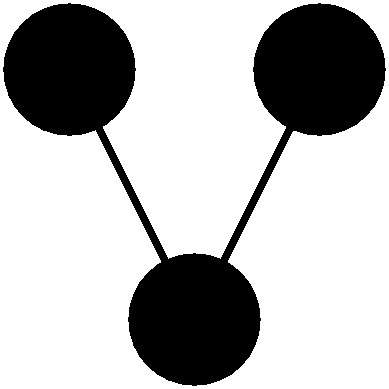
\epsfig{file = ../figures/Vmotif.eps, width=.3cm, clip=} &
      14\,113 & 13\,118 & 2\,599 & 3E${-1}$ \\ 
      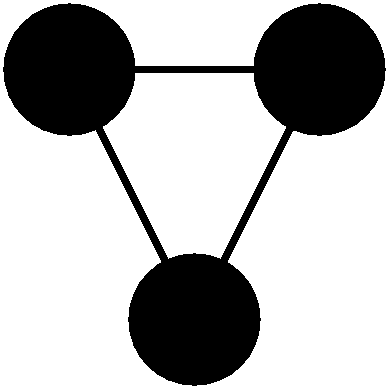
\epsfig{file = ../figures/trianglemotif.eps, width=.3cm, clip=}
      & 75 & 64.4 & 20 & 3E${-1}$ \\ 
      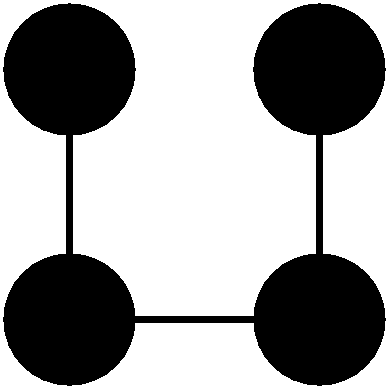
\epsfig{file = ../figures/chainmotif.eps, width=.3cm, clip=} &
      98\,697 & 90\,059 & 26\,064 & 3E${-1}$ \\ 
      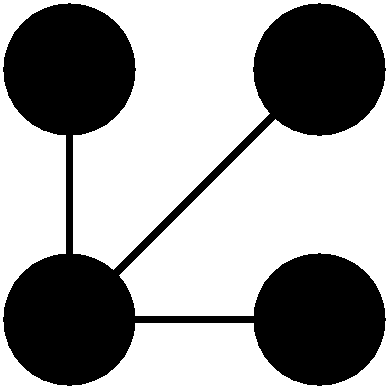
\epsfig{file = ../figures/starmotif.eps, width=.3cm, clip=} &
      112\,490 & 89\,372 & 26\,423 & 2E${-1}$ \\
      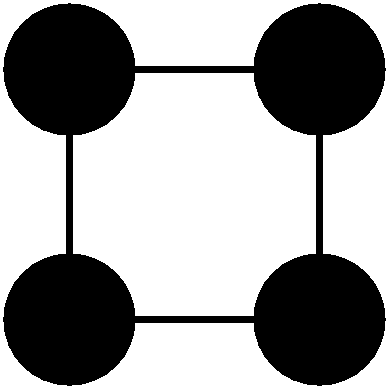
\epsfig{file = ../figures/squaremotif.eps, width=.3cm, clip=} &
      1\,058 & 492 & 202 & \emphase{1E${-2}$} \\ 
      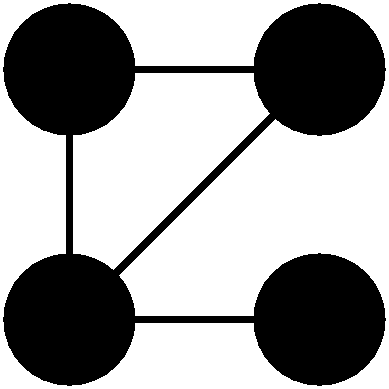
\epsfig{file = ../figures/whisker.eps, width=.3cm, clip=} &
      3\,535 & 2\,756 & 1\,087 & 2E${-1}$ \\ 
      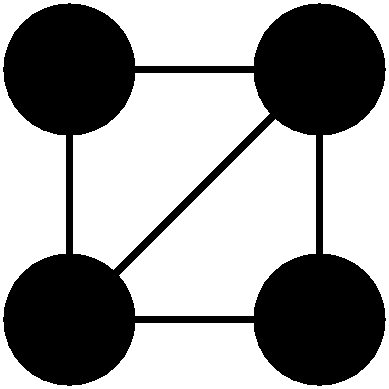
\epsfig{file = ../figures/halfclique.eps, width=.3cm, clip=} & 79 &
      33.2 & 19.5 & \emphase{3E${-2}$} \\ 
      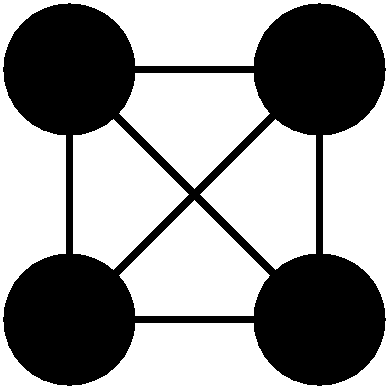
\epsfig{file = ../figures/clique.eps, width=.3cm, clip=} & 0 &
      0.165 & 0.432 & 1.00 \\ 
    \end{tabular}
    }
    &
    \hspace{-.6cm}
    {\small
    \begin{tabular}{rrrr} 
      $N_{\obs}(\mbf)$ &
      $\overline{N}_{100}$&$\overline{\sigma }_{100}$&
      $p$ \\
      \hline
      13\,888 & {13\,648} & {51.8} &  {2E${-6}$}    \\
      75      & {155}   & {17.3} & {2E${-6}$}     \\
      87\,869 & {112\,532} & {1\,957} & {1E${-36}$}  \\
      109\,113& {103\,186} & {1\,084} & {2E${-8}$}     \\
      979     & {796} & {64.7} & {2E${-3}$}    \\
      3\,219  & {8\,734} & {945} & {3E${-9}$}   \\
      79      & {273} & {66.7}& {2E${-3}$}    \\
      0       & {6.2} & {3.7} & {4E${-2}$}       
    \end{tabular}
    }
  \end{tabular}
  }

%==================================================================== 
\section{Extensions \& Open Questions} 
\subsection*{Network comparison}
\frame{ \frametitle{Extensions \& Open Questions} \pause
%  \frametitle{Network description} 
%==================================================================== 
  \paragraph{Network comparison:} under (H1) and (H2), in a graph $g$,
  we have
  $$
  \Esp N_g(\mbf) = \binom{n_g}{k_m} \mu_g(\mbf)
  \qquad \Rightarrow \qquad
  \tilde{N}_g(\mbf) := \binom{n_g}{k_m}^{-1} N_g(\mbf).
  $$

  \bigskip
  \paragraph{Vector of normalised counts:} for a given set of motifs
  $\{\mbf_m\}_m$, a network $g$ can be described by counts
  $$
  \tilde{\Nbf}_g = [\tilde{N}(\mbf_1) \; \dots \; \tilde{N}(\mbf_M)].
  $$
  the moments of which are
  $$
  \mubf_g := \Esp(\tilde{\Nbf}_g)
  \qquad \text{and} \qquad
  \tilde{\Sigmabf}_g := \Var(\tilde{\Nbf}_g).
  $$
  If networks $g$ and $g'$ are independent,
  $$
  \Esp(\tilde{\Nbf}_g - \tilde{\Nbf}_{g'}) = \mubf_g - \mubf_{g'}, 
  \qquad
  \Var(\tilde{\Nbf}_g - \tilde{\Nbf}_{g'}) = \tilde{\Sigmabf}_g +
  \tilde{\Sigmabf}_{g'} 
  $$
  }

%==================================================================== 
\frame{ \frametitle{Network comparison}
  \begin{tabular}{cc}
    \hspace{-.5cm}
    \begin{tabular}{p{.5\textwidth}}
      \paragraph{Mahalanobis distance:} 
      %This suggest to define
      $$
      d^2(g, g') = \|\tilde{\Nbf}_g - \tilde{\Nbf}_{g'}
      \|^2_{(\tilde{\Sigmabf}_g + \tilde{\Sigmabf}_{g'})^{-1}}.
      $$
      
      \bigskip
      \paragraph{Question:} What is the (approximate) distribution of
      $d^2(g, g')$ under 
      $$      
      \Hbf_0 = \{\mubf_g = \mubf_{g'}\}
      $$
    \end{tabular}
    &
    \begin{tabular}{p{.45\textwidth}}
    \hspace{-.5cm}
      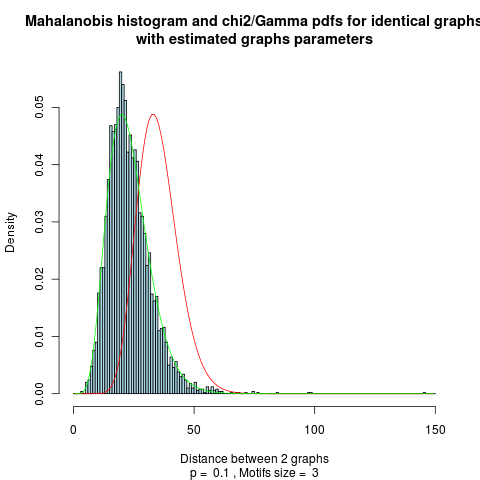
\epsfig{file =
      ../Figures/MahalanobisHist_EstimatedParam_p0.1_AllMotifsSize3.ps,
      clip=, width=.45\textwidth} 
    \end{tabular}
  \end{tabular} \\
  (Work in progress by \textcolor{blue}{\sl L. Benaroya}) 
  }

%==================================================================== 
\frame{ \frametitle{Extensions}
  \paragraph{Accounting for covariates}
  \begin{itemize}
  \item Host/parasite network: $X_{ij} = $ number of parasites (hosts)
    shared by species $i$ and $j$.
  \item Does the phylogenetic between species proximity contribute
    to the existence of clusters?
  \item Possible to combine mixture and generalised linear models.
  \end{itemize}

  \bigskip\bigskip
  \paragraph{Other motifs}
  \begin{itemize}
  \item Metabolic network: node = enzyme, belonging to a known
    category (color),
  \item Colored motif = connected sub-graph with given colors,
  \item Moments $\Esp[N(\mbf)]$ and $\Var[N(\mbf)]$ known for the
    colored Erd�s model.
  \end{itemize}
   
  }

%==================================================================== 
\frame{ \frametitle{Some open questions}
  \paragraph{(Asymptotic) distributions}
  \begin{itemize}
  \item of the counts $N(\mbf)$,
  \item of the distance $d(g, g')$,
  \end{itemize}
  for non-naive random graph models.

  \bigskip\bigskip
  \paragraph{Accounting for parameter estimation} 
  \begin{itemize}
  \item Even for the Erd�s model, $\thetabf$ has to be  estimated ...
  \item Often on the same graph where $N(\mbf)$ is counted.  
  \end{itemize}
  }

%====================================================================

%====================================================================
%====================================================================
\frame{ \frametitle{References}
  \tiny{
    \bibliographystyle{/Latex/astats}
    \bibliography{/Biblio/AST,/Biblio/SSB,/Biblio/ARC}
    }
  }
%====================================================================


%====================================================================
%====================================================================
\section*{Variational Bayes inference}
\subsection*{Bayesian inference}
\frame{ \frametitle{Variational Bayes inference} \pause
%==================================================================== 
  \paragraph{Bayesian point of view:} The parameter $\thetabf$ itself
  {is random}:
  $$ 
  \thetabf \sim P(\thetabf)
  $$
  where $P(\thetabf)$ is {prior} distribution of $\thetabf$.

  \bigskip
  \paragraph{Bayesian inference:} The goal is then to calculate the
  {posterior} distribution
  $$
  P(\thetabf|\Xbf) = \frac{P(\thetabf) P(\Xbf|\thetabf)}{P(\Xbf)}.
  $$
  \begin{itemize}
  \item Its explicit calculation is possible in nice cases, e.g.
    exponential family with conjugate prior.
  \item Monte-Carlo (e.g. MCMC) sampling is often used to estimate it.
  \end{itemize}
  }

%==================================================================== 
\frame{\frametitle{Incomplete data model}
  \paragraph{Hierarchical modelling:} The model is typically defined
  with:
  $$
  \begin{tabular}{ll}
    the prior distribution of $\thetabf$: & \emphase{$P(\thetabf)$} \\
    \\
    the conditional distribution of the unobserved $\Zbf$: &
    \emphase{$P(\Zbf|\thetabf)$} \\
    \\
    the conditional distribution of the observed $\Xbf$: &
    \emphase{$P(\Xbf|\Zbf, \thetabf)$}
  \end{tabular}
  $$

  \bigskip
  \paragraph{Inference:} The goal is know to calculate (or estimate)
  the {joint conditional distribution}
  $$
  P(\Zbf, \thetabf|\Xbf) = \frac{P(\thetabf) P(\Zbf|\thetabf)
    P(\Xbf|\Zbf, \thetabf)}{P(\Xbf)}
  $$
  which is often {intractable}, even when $P(\Zbf|\Xbf,
  \thetabf)$ can be calculated (e.g. independent mixture models).
  }

%==================================================================== 
\subsection*{VB-EM}
%==================================================================== 
\frame{ \frametitle{Variational Bayes inference}
  \paragraph{Exponential family / conjugate prior:} if
  \begin{eqnarray*}
    \log P(\thetabf) & = & \phi(\thetabf)^\intercal \nubf + \cst \\
    \log P(\Xbf, \Zbf | \thetabf) & = & \phi(\thetabf)^\intercal
    u(\Xbf, \Zbf) + \cst. 
  \end{eqnarray*}

  \bigskip
  \paragraph{Variational optimisation:} The best approximate distribution
  $$
  Q^* = \arg\min_{Q \in \Qcal} KL[Q(\Zbf, \thetabf); P(\Zbf,
  \thetabf | \Xbf)]
  $$
  within the class of \emphase{factorisable distributions} $\Qcal$:
  $$
  \Qcal = \{Q: Q(\Zbf, \thetabf) = Q_Z(\Zbf)Q_\theta(\thetabf)\}
  $$
  can be recovered via a {variational Bayes E-M algorithm (VBEM)}
  [\refer{BeG03}]. 
}

%==================================================================== 
\frame{ \frametitle{VB-EM algorithm} 
  
  The approximate conditional distributions $Q_Z(\Zbf)$ and
  $Q_\theta(\thetabf)$ are alternatively updated.

  \paragraph{VB-M step:} Approximate posterior of $\thetabf$
  $$
  \log Q(\thetabf) = \phi(\thetabf)^\intercal \left\{\Esp_{Q_Z}[u(\Xbf,
    \Zbf)] + \nubf\right\} + \cst
  $$
  \paragraph{VB-E step:} Approximate conditional distribution of $\Zbf$
  $$
  \log Q(\Zbf) = \Esp_{Q_\theta}[\phi(\thetabf)]^\intercal u(\Xbf,
  \Zbf) + \cst
  $$

  \bigskip
  \paragraph{General properties:} Still not well known
  \begin{itemize}
  \item Consistency for some particular cases.
  \item Generally tend to underestimate the posterior variance of
    $\thetabf$.
  \item Obviously depends on the quality of the approximate
    $Q(\thetabf, \Zbf)$.
  \end{itemize}
  }

%==================================================================== 
\subsection*{Mixture for networks}
%==================================================================== 
\frame{ \frametitle{Application to mixtures for networks}
  \paragraph{VB-EM Credibility intervals} with a mixture of 2 groups of nodes\\
  ~\\
  \includegraphics[width=1\textwidth]{/ENSEIGN/COURS/MELANGE/Exposes/Figures/im-ICQ2-2-new} \\
  $\pi_1$: $+$, $\gamma_{11}$: \textcolor{red}{$\triangle$},
  $\gamma_{12}$: \textcolor{blue}{$\circ$}, $\gamma_{22}$:
  \textcolor{green}{$\bullet$}

  \begin{itemize}
  \item For all parameters, VB-EM posterior credibility intervals
    achieve the nominal level (90\%), as soon as $n \geq 25$.
  \item \emphase{$\rightarrow$} the VB-EM approximation works well, at least for
    graphs.
  \end{itemize}
  }

%====================================================================
\frame{ \frametitle{Approximate posterior distribution}
%==================================================================== 
  \vspace{-1cm}\hspace{-.5cm}
  \begin{tabular}{cc}
    \begin{tabular}{c}
      \includegraphics[width=.5\textwidth]{/ENSEIGN/COURS/MELANGE/Exposes/Figures/im-pi1BVEM}\\         
      \includegraphics[width=.5\textwidth]{/ENSEIGN/COURS/MELANGE/Exposes/Figures/im-pi2BVEM}\\
      \includegraphics[width=.5\textwidth]{/ENSEIGN/COURS/MELANGE/Exposes/Figures/im-pi3BVEM}\\
      \includegraphics[width=.5\textwidth]{/ENSEIGN/COURS/MELANGE/Exposes/Figures/im-pi4BVEM}\\
      \includegraphics[width=.5\textwidth]{/ENSEIGN/COURS/MELANGE/Exposes/Figures/im-pi5BVEM}\\
      \hline \\
      \includegraphics[width=.5\textwidth]{/ENSEIGN/COURS/MELANGE/Exposes/Figures/im-alphaBVEM}\\
    \end{tabular}
    &
    \begin{tabular}{c}
      \hspace{-.5cm}
      \includegraphics[width=.5\textwidth]{/ENSEIGN/COURS/MELANGE/Exposes/Figures/im_EcoliBVEM} \\
    \end{tabular}
  \end{tabular}  
  }


%====================================================================
%====================================================================
\end{document}
%====================================================================
%====================================================================
